\section{System representations}

The discrete-time dynamic linear system is represented by the following block diagram:
\begin{figure}[H]
    \centering
    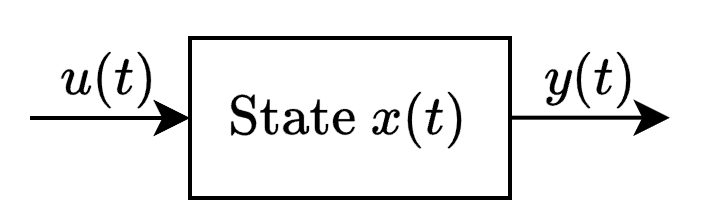
\includegraphics[width=0.4\linewidth]{images/rep.png}
\end{figure}

\subsection{State space representation}
State space (or internal) representation describes a system where the state $x(t)$ comprises internal variables known as states. 
The system can be represented as:
\[\begin{cases}
    x(t+1)=Fx(t)+Gu(t) \\
    y(t)=Hx(t)+Du(t)
\end{cases}\]
Here, $x(t+1)=Fx(t)+Gu(t)$ is termed the state equation, a difference equation, and $y(t)=Hx(t)+Du(t)$ is the output equation.
In the case of a single input single output system, $F$ (state matrix) is an $n \times n$ matrix, $G$ (input matrix) is an $n \times 1$ column vector, $H$ (output matrix) is a $1 \times n$ row vector, and $D$ (input-output matrix) is a scalar. 
\begin{definition}[\textit{Strictly proper system}]
    A system is termed strictly proper if the input doesn't directly affect the output.
\end{definition}
\begin{property}
    The system is strictly proper if the matrix $D$ is zero. 
\end{property}    
\begin{property}
    The system is stable if the eigenvalues of the matrix $F$ lie within the unit circle.
\end{property}
\begin{example}
    Let's consider the following single input single output system of order two:
    \[\begin{cases}
        x_1(t+1)=\frac{1}{2}x_1(t)+2u(t) \\
        x_2(t+1)=x_1(t)+2x_2(t)+u(t) \\
        y(t)=\frac{1}{4}x_1(t)+\frac{1}{2}x_2(t)
    \end{cases}\]
    The characteristic matrices are:
    \[F=\begin{bmatrix} \frac{1}{2} & 0 \\ 1 & 2 \end{bmatrix} \quad G=\begin{bmatrix} 2 \\ 1 \end{bmatrix} \quad H=\begin{bmatrix} \frac{1}{4} & \frac{1}{2} \end{bmatrix} \quad D=\begin{bmatrix} 0 \end{bmatrix}\]
    As the matrix $F$ is diagonal, its eigenvalues are $\frac{1}{2}$ and $2$, indicating instability.
\end{example}
The state space representation of the system is not unique. 
We can transform it as follows:
\[\begin{cases}
    F \rightarrow F_1 = T_1 F T_1^{-1} \\ 
    G \rightarrow T_1 G \\
    H \rightarrow H T_1^{-1} \\ 
    D \rightarrow D
\end{cases}\]
These representations are equivalent for all invertible square matrices $T_1$, where $T_1$ is an $n \times n$ matrix.

\subsection{Transfer function representation}
The transfer function (or external) representation is derived from the input/output time domain difference equation by utilizing the delay operator $z^{-1}$: 
\[z^{-1}x(t)=x(t-1) \qquad z^{1}x(t)=x(t+1)\]
\begin{example}
    Consider the following time domain difference equation:
    \[y(t)=-\dfrac{1}{6}y(t-1)-\dfrac{1}{8}y(t-2)+\dfrac{1}{2}u(t-1)+\dfrac{1}{4}u(t-2)\]
    Using the time shift operator, we bring all the signals to the base time $t$: 
    \[y(t)=-\dfrac{1}{6}y(t)z^{-1}-\dfrac{1}{8}y(t)z^{-2}+\dfrac{1}{2}u(t)z^{-1}+\dfrac{1}{4}u(t)z^{-2}\]
    By collecting the terms, we get:
    \[y(t)=\dfrac{\frac{1}{2}z^{-1}+\frac{1}{4}z^{-2}}{1+\frac{1}{6}z^{-1}-\frac{1}{8}z^{-2}}u(t)\]
    Where the fractional term is the transfer function $W(z)$ from the input $u(t)$ to output $y(t)$. 

    We can also transform the transfer function into its positive power representation:
    \[W(z)=\dfrac{\frac{1}{2}z+\frac{1}{4}}{z^2+\frac{1}{6}-\frac{1}{8}}\]
\end{example}
In general we have: 
\begin{figure}[H]
    \centering
    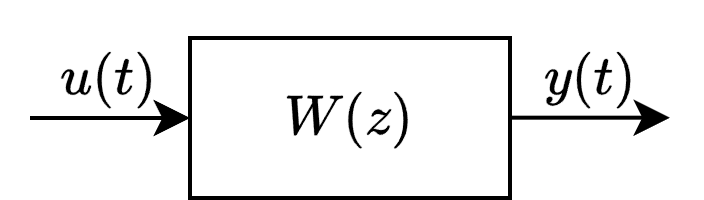
\includegraphics[width=0.4\linewidth]{images/transfer.png}
\end{figure}
In general, the transfer function can be represented as:
\[W(z)=\dfrac{B(z)}{A(z)}z^{-k}=\dfrac{b_0+b_1 z^{-1}+\cdots+b_p z^{-p}}{a_0+a_1 z^{-1}+\cdots+a_n z^{-n}}z^{-k}\]
\begin{property}
    The system is strictly proper if the time delay $k$ is greater than or equal to one.
\end{property}    

\subsection{Impulse response representation}
This representation, also known as convolution of the input with the impulse response, relies on the impulse in discrete time, which has a value of one at time zero and null values at all other instants.

The response of the system at successive instants starting from zero constitutes the impulse response $\omega(t)$: 
\[\text{impulse response}=\left\{ \omega(0),\omega(1),\omega(2),\omega(3),\dots \right\}\]
The output of the system can be expressed as:
\[y(t)=\omega(0)u(t)+\omega(1)u(t-1)+\omega(2)u(t-2)+\omega(3)u(t-3)+\cdots=\sum_{k=0}^{+\infty}\omega(k)u(t-k)\]
Thus, the output $y(t)$ is the convolution of the generic input signal $u(t)$ with the impulse response coefficients.

\paragraph*{Filters}
The filter: 
\[W(z)=\dfrac{z^{-1}+\frac{1}{2}z^{-2}}{1+\frac{1}{3}z^{-1}}\]
is termed an Infinite Impulse Response Filter.

The filter: 
\[W(z)=z^{-1}+\dfrac{1}{2}z^{-2}+\dfrac{1}{3}z^{-3}\]
is referred to as a finite impulse response filter.